\chapter{Directed deformation retracts and the dihomotopy hypothesis}
\label{chap:modstr}




\section{The homotopy hypothesis}
	
%	The homotopy hypothesis is a folklore result in algebraic topology which states that $\infty$-groupoids reflect exactly the algebraic structure of a topological space \cite{grothendieck83}. 

The homotopy hypothesis is a test to apply to any potential model for $\infty$-groupoids: any reasonable interpretation  of what $\infty$-groupoids are should reflect exactly the algebraic structure of a topological space \cite{grothendieck83}. Intuitively, a (small) $\infty$-category is a set of objects (of dimension $0$), between every pair of objects a set of morphisms (objects of dimension $1$), between every pair of morphisms between two objects a set of $2$-morphisms (objects of dimension $2$), and so on. An $\infty$-groupoid is then an $\infty$-category where all those data are invertible up to higher-dimensional data.
	
	A topological space intuitively naturally gives rise to a structure of $\infty$-category. Its $0$-dimensional objects are points, its $1$-dimensional are paths, its $2$-dimensional objects are homotopies (i.e., paths in the space of paths), and so on. All those data are invertible, that is, form a $\infty$-groupoid: for example, we have seen that paths have an inverse modulo homotopy. 
	
	The homotopy hypothesis states that to study the geometry of a topological space, up to continuous deformations, it should be enough to study this $\infty$-groupoid, whatever the reasonable interpretation chosen for the latter.
	
	A modern formulation of the homotopy hypothesis uses the language of model categories, introduced in \cite{quillen67}. Model structures are a convenient framework to design theories of certain objects modulo weak-equivalences, namely morphisms that are not necessarily isomorphisms but, in a way, act as such. They give nice conditions for the localization to be defined and computable in some way. They also allow one to compare those structures by comparing their localizations. In this section, we start be recalling definitions in model structures: lifting property, weak factorization system, homotopy, Quillen-equivalence (Section \ref{subsec:modstr}). In parallel, we will follow the example of the Str\o m model structure: a model structure on topological spaces whose weak-equivalences are homotopy equivalences.
	
	After that, in Section \ref{subsec:quiser}, we will see another model structure in topological spaces, the Quillen-Serre model structure, whose weak-equivalences are weak homotopy equivalences, namely continuous functions that induce isomorphisms between homotopy groups. That is precisely this model structure that will be reflected by $\infty$-groupoids. In the language of model structures, this means that we will present a model structure, the Kan-Quillen model structure, which models $\infty$-groupoids and that will be Quillen-equivalent to the Quillen-Serre model structure. It will be based on simplicial sets (Section \ref{subsec:simset}) and its fibrant and cofibrant objects, the Kan complexes (Section \ref{subsec:kancom}) are precisely the objects that model $\infty$-groupoids.
	
	\subsection{Model structures}
	\label{subsec:modstr}
	
	A model structure on a category is given by three classes of morphisms: the weak-equivalences, that almost act like isomorphisms, typically like isomorphisms up to homotopy ; fibrations that act like nice surjections lifting things, typically lifting homotopies ; cofibrations that act like nice injections extending things, typically extending homotopies. Those three classes of morphisms will satisfies some properties that will allow the computation of the localization at the week-equivalence: it will be equivalent to a category of homotopy types and morphisms up to homotopy. This localization is precisely what we mean by modeling something: for example, a model for $\infty$-groupoids will be a such a localization such that its objects act like $\infty$-groupoids. It will also be possible to compare model structures with the notion of Quillen-equivalences, forcing model structures to have the same localization.
	
		\subsubsection{Lifting property}
	
	The conditions on those data will be based on fibrational properties, meaning that they will use morphisms having lifting properties with respect to others. We say that a morphism $\map{f}{a}{b}$ has the \textbf{left lifting property} with respect to $\map{g}{c}{d}$ (or equivalently, that $g$ has the \textbf{right lifting property} with respect to $f$) if for every commutative diagram of the form:
	\begin{center}
	\begin{tikzpicture}[scale=2]
		\node (A) at (0,1) {$a$};
		\node (B) at (1.2,1) {$c$};
		\node (C) at (0,0) {$b$};
		\node (D) at (1.2,0) {$d$};
		\path[->,font=\scriptsize]
		(A) edge node[above]{$u$} (B)
		(A) edge node[left]{$f$} (C)
		(C) edge node[below]{$v$} (D)
		(B) edge node[right]{$g$} (D);
	\end{tikzpicture}
	\end{center}
	there is a morphism $\map{\theta}{b}{c}$ which makes the following  diagram commutes:
	\begin{center}
	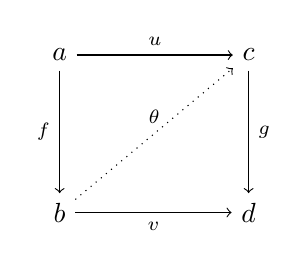
\begin{tikzpicture}[scale=2]
		\node (A) at (0,1) {$a$};
		\node (B) at (1.2,1) {$c$};
		\node (C) at (0,0) {$b$};
		\node (D) at (1.2,0) {$d$};
		\path[->,font=\scriptsize]
		(A) edge node[above]{$u$} (B)
		(A) edge node[left]{$f$} (C)
		(C) edge node[below]{$v$} (D)
		(B) edge node[right]{$g$} (D);
		\path[->,font=\scriptsize, dotted]
		(C) edge node[above]{$\theta$} (B);
	\end{tikzpicture}
	\end{center}
	
	A crucial example in topological space is the \textbf{homotopy lifting property}. We say that a continuous function $\map{f}{X}{Y}$ has the homotopy lifting property with respect to $Z$ if and only if for every continuous function $\map{g}{Z}{X}$ and every classical homotopy $\map{H}{Z\times [0,1]}{Y}$ such that $H(z,0) = f\circ g(z)$, then there is a classical homotopy $\map{K}{Z\times[0,1]}{X}$ such that $K(z,0) = g(Z)$ and $H = f\circ K$. Equivalently, $f$ has the homotopy lifting property with respect to $Z$ if and only if it has the right lifting property with respect to $\map{\iota_0}{Z}{Z\times[0,1]}$, which maps $z$ to $(z,0)$. We call \textbf{Hurewicz fibration} (resp. \textbf{Serre fibration}) any function which has the homotopy lifting property with respect to every space (resp. with respect to every cube $\Box_n$).
	
	Dually, we say that a continuous function $\map{f}{X}{Y}$ has the \textbf{homotopy extension property} with respect to $Z$ if and only if for every function $\map{g}{Y}{Z}$ and every homotopy $\map{H}{X}{P(Z)}$ such that $H(x)(0) = g\circ f(x)$, then there is a homotopy $\map{K}{Y}{P(Z)}$ such that $K(y)(0) = g(y)$ and $K\circ f = H$. Equivalently, $f$ has the homotopy extension property with respect to $Z$ if and only if it has the left lifting property with respect to $\map{\sigma_0}{P(Z)}{Z}$ which maps every path $\gamma$ to $\gamma(0)$. We call \textbf{Hurewicz cofibration} any function which has the homotopy extension property with respect to every space.
	
	
		\subsubsection{Model categories}
	
By a \textbf{weak factorization system} on $\C$, we will mean a pair $(L,R)$ of classes of morphisms such that:
	\begin{itemize}
		\item every morphisms $\map{f}{a}{b}$ of $\C$ can be factorized as:
		$$a \xrightarrow{~~ \in L ~} c \xrightarrow{~~ \in R ~~} b,$$
		\item $L$ is precisely the class of morphisms of $\C$ which have the left lifting property with respect to every element of $R$,
		\item $R$ is precisely the class of morphisms of $\C$ which have the right lifting property with respect to every element of $L$.
	\end{itemize}
	
	
	
	A \textbf{model category} is a complete and cocomplete category $\C$ together with three classes of morphisms:
	\begin{itemize}
		\item $W$ called \textbf{weak equivalences},
		\item $\fib$ called \textbf{fibrations},
		\item $\cof$ called \textbf{cofibrations},
	\end{itemize}
	satisfying that:
	\begin{itemize}
		\item $W$ makes $\C$ into a category with weak equivalences. Recall that this means that every isomorphism of $\C$ is in $W$ and $W$ has the 2-out-of-3 property.
		\item $(\cof,\fib\cap W)$ and $(\cof\cap W, \fib)$ are weak factorization systems on $\C$.
	\end{itemize}
	
	For example, $\topo$ with homotopy equivalences as weak equivalences, Hurewicz fibrations as fibrations, and closed Hurewicz cofibrations, i.e., Hurewicz cofibrations $\map{f}{X}{Y}$ such that $f(X)$ is closed in $Y$, as cofibrations form a model category called the \textbf{Str\o m model category} \cite{strom72}.
	
	
	We say that an object $c$ is \textbf{fibrant} if the unique morphism from $c$ to the final object of $\C$ is a fibration. Dually, we say that it is \textbf{cofibrant} if the unique morphism from the initial object to $c$ is a cofibration. The fibrant cofibrant objects are of particular interest: since every $c$ is weakly equivalent to a fibrant cofibrant object, those objects can be thought as ``homotopy types'' of objects. In the case of the Str\o m model structure, every space is fibrant and cofibrant, but this a very particular property from this model category.
	
	
	\subsubsection{Homotopy and homotopy category}
	
	In a model category, there always is a notion of homotopy, using a cylinder object (that you can think as the product by a segment, for example $X\times [0,1]$ is a cylinder object). A \textbf{cylinder object} of an object $X$ in a model category is an object $\text{Cyl}(X)$ such that the codiagonal map $\map{\Delta_X}{X\sqcup X}{X}$ factorizes as:
	$$X\sqcup X \xrightarrow{~~ \iota ~~} \text{Cyl}(X) \xrightarrow{~~ p ~~} X$$
	where $p$ is a weak equivalence. A \textbf{left homotopy} from $f$ to $g$, where $\map{f,g}{X}{Y}$ is a map $H$ from any cylinder object $\text{Cyl}(X)$ to $Y$ such that $H \circ \iota = f\sqcup g$.
	
	In a model category, this notion of homotopy is an equivalence relation. It coincide with a dual notion of \textbf{right homotopy} using \textbf{path objects} instead (for example, the space of paths). In the case of Str\o m model structure, left and right homotopies coincide with (classical) homotopy. The interest of this is that, between cofibrant and fibrant objects, weak equivalences coincide with homotopy equivalences, that is, maps that are invertible up to left homotopy. This implies in particular that the localization $\loca{\C}{W}$ is equivalent to the category whose objects are fibrant and cofibrant objects and whose morphisms are morphisms of $\C$ modulo left homotopy. This category, noted $\textbf{Ho}(\C)$, is called the \textbf{homotopy category} of $\C$. Coherently, the homotopy category $\hotop$ is the homotopy category of the Str\o m model category.
	
	The language of model categories provides also a way to compare those models, by giving some condition for the homotopy categories to be equivalent. A \textbf{Quillen adjunction} $F \dashv G$ from a model category $\C$ to $\C'$ is an adjunction such that $F$ maps cofibrations of $\C$ to cofibrations of $\C'$ and $G$ maps fibrations of $\C'$ to fibrations of $\C$. A \textbf{Quillen equivalence} is a Quillen adjunction such that for every cofibrant object $c$ of $\C$ and every fibrant object $c'$ of $\C'$, a maps from $c$ to $G(c')$ is a weak equivalence of $\C$ if and only if the adjoint morphism from $F(c)$ to $c'$ is a weak equivalence of $\C'$. The interest is that a Quillen equivalence induces an equivalence of categories between the homotopy categories $\textbf{Ho}(\C)$ and $\textbf{Ho}(\C')$.
	
	
	
	
	
	
		
		
	\subsection{Quillen-Serre model structure}
	\label{subsec:quiser}
	
	
	Actually, the Str\o m model category is folklore and was not the first one considered by Quillen. It has no particular interest except to make things coherent. The first model category was a model category on $\topo$ whose weak equivalences are \textbf{weak homotopy equivalences}. Those are continuous functions that induces isomorphisms between \textbf{homotopy groups}. We have seen that a homotopy equivalence induces an equivalence of categories between fundamental groupoids. Given a topological space $X$, and a point $x$ of $X$, the homset $\pi_1(X)(x,x)$, denoted $\pi_1(X,x)$, is then a group and is called the \textbf{first homotopy group of $X$}. A homotopy equivalence $\map{f}{X}{Y}$ induces an isomorphism of groups $\map{\pi_1(f)}{\pi_1(X,x)}{\pi_1(Y,f(x))}$. This homotopy group can be expressed directly. Denote by $\topp$ the category whose objects are pairs $(X,A)$ of topological spaces with $A \subseteq X$, and whose morphisms from $(X,A)$ to $(Y,B)$ are continuous functions $\map{f}{X}{Y}$ with $f(A) \subseteq B$. Given two maps $\map{f,g}{(X,A)}{(Y,B)}$, a \textbf{homotopy relative to} $A$ is a map $\map{H}{(X\times [0,1],A\times[0,1])}{(Y,B)}$ such that $H(x,0) = f(x)$ and $H(x,1) = g(x)$. A \textbf{relative homotopy class} of a map $f$ in $\topp$ will be the class of maps that are homotopic to $f$. $\pi_1(X,x)$ is then the set of homotopy classes of maps from $(\Box_1 = [0,1],\partial\Box_1 = \{0,1\})$ to $(X,x)$, with concatenation as group operation. This can be generalized to any dimension: denote by $\pi_n(X,x)$ the set of homotopy classes of maps from $(\Box_n,\partial\Box_n)$, where $\partial\Box_n$ is the subspace of $\Box_n$ whose points are $(t_1, \ldots, t_n)$ such that there is $i \in \{1,\ldots, n\}$ with $t_i \in \{0,1\}$, to $(X,x)$. There are several ways to define a group operation on $\pi_n(X,x)$: fix $i \in \{1,\ldots, n\}$ and $\map{f,g}{(\Box_n,\partial\Box_n)}{(X,x)}$. Define $\map{f\star_i g}{(\Box_n,\partial\Box_n)}{(X,x)}$ as 
		\begin{align*}
			f\star_i g(t_1, \ldots, t_n) 	&	=  f(t_1, \ldots, t_{i-1}, 2t_i, t_{i+1}, \ldots, t_n)& \text{ if } t_i\leq \frac{1}{2}\\
      				 					&	= g(t_1, \ldots, t_{i-1}, 2t_i-1, t_{i+1}, \ldots, t_n)& \text{ if } t_i\geq \frac{1}{2}
		\end{align*}
By an Eckmann-Hilton argument, those operations coincide and are commutative which makes $\pi_n(X,x)$ Abelian groups for $n \geq 2$. Finally, denote by $\pi_0(X)$ the set of path-connected components of $X$. All those data are functorial, that is, a continuous function $\map{f}{X}{Y}$ induces a group morphism (resp. a function) from $\pi_n(X,x)$ to $\pi_n(Y,f(x))$ for $n \geq 1$ (resp. from $\pi_0(X)$ to $\pi_0(Y)$). We say that $f$ is a \textbf{weak homotopy equivalence} if those morphisms are isomorphisms. In particular, a homotopy equivalence is a weak homotopy equivalence.


There is a model category on $\topo$ whose weak equivalences are weak homotopy equivalences, called the Quillen-Serre model structure. See \cite{quillen67} for a description and proofs. In this model category, the fibrations are Serre fibrations and the fibrant and cofibrant objects are the so-called \textbf{CW-complexes}. The identity functor on $\topo$ forms a Quillen-adjunction from Str\o m model structure to Quillen-Serre model structure.
		
		
		
\subsection{A modern formulation of the homotopy hypothesis}
		\label{subsec:hohy}
		
		
		\subsubsection{Simplicial sets}
		\label{subsec:simset}
		
		In this section, we present a model for $\infty$-groupoids, which, in retrospect, can be seen to be inherent in work even before the formulation by Grothendieck of the homotopy hypothesis in 1983; see for instance in Quillen's lecture notes \cite{quillen67}. They are defined as particular \textbf{simplicial sets}. Simplicial sets are similar to precubical sets, in the sense that they are particular presheaves. Define the category $\Delta$ whose objects are integers and whose morphisms from $n$ to $m$ are monotonous functions $\map{f}{\{0,\ldots, n\}}{\{0,\ldots,m\}}$. Among those maps, there are two particular types of functions of particular interest:
		\begin{itemize}
			\item for $n \in\nat$ and $i \in \{0,\ldots, n+1\}$, $\map{\delta_i}{n}{n+1}$ which maps $j < i$ to $j$ and $j \geq i$ to $j+1$. They are called \textbf{face maps}.
			\item for $n \in \nat$ and $i \in \{0,\ldots, n\}$, $\map{\sigma_i}{n+1}{n}$ which maps $j \leq i$ to $j$ and $j > i$ to $j-1$. They are called \textbf{degeneracy maps}.
		\end{itemize}
		
		A \textbf{simplicial set} is a functor from $\Delta^{op}$ to $\setcat$, i.e., a presheaf on $\Delta$. Since face and degeneracy maps generate the category $\Delta$, there is a more practical definition of simplicial sets. A simplicial set is a collection $(X_n)_{n\in \nat}$ of sets together with functions:
		\begin{itemize}
			\item for every $n \in \nat$, for every $i \in \{0,\ldots, n+1\}$, $\map{d_i}{X_{n+1}}{X_n}$, also called \textbf{face maps}.
			\item for every $n \in \nat$, for every $i \in \{0,\ldots,n\}$, $\map{s_i}{X_n}{X_{n+1}}$, also called \textbf{degeneracy maps}.
		\end{itemize}
		satisfying the following equations, called the \textbf{simplicial relations}:
		\begin{align*}
			d_i\circ d_j 			& =  d_{j-1}\circ d_i 				& \text{ if } i < j\\
      			s_i\circ s_j	 			& = s_{j+1}\circ s_i				& \text{ if } i \leq j\\
			d_i\circ s_j			& = \text{id}					& \text{ if } i \in \{j,j+1\}\\
			d_i\circ s_j			& = s_j\circ d_{i-1}				& \text{ if } i > j+1\\
			d_i\circ s_j			& = s_{j-1}\circ d_i				& \text{ if } i < j
		\end{align*}
		
		A morphism of simplicial sets from $X$ to $X'$ is a natural transformation from $X$ to $X'$, seen as functors. More practically, it is a collection of morphisms $(\map{f_n}{X_n}{X'_n})_{n\in\nat}$ such that:
		$$f_n \circ d_i = d'_i \circ f_{n+1}$$
		$$f_{n+1}\circ s_i = s'_i \circ f_n$$
		We denote by $\sset$ the category of simplicial sets and morphisms of simplicial sets.
		
		
		
		\subsubsection{Geom-Sing adjunction}
		
		Much as in precubical sets, a functor $\map{F}{\Delta}{\C}$ with $\C$ cocomplete induces a functor $\map{\tilde{F}}{\sset}{\C}$ which has automatically a right adjoint. This allows one to nicely construct a geometric realization of a simplicial set. For $n \in \nat$, let $\Delta_n$ be the subspace of $\mathbb{R}^{n+1}$ whose points are the $(t_0,\ldots,t_n)$ such that $t_i \in [0,1]$ and $\sum\limits_{i = 0}^n t_i = 1$. Those spaces are called \textbf{standard geometric simplexes}. 
		
			\begin{figure}[H]
			\begin{center}
				\begin{tikzpicture}[auto,scale = 0.7]
\draw (0,0.5) -- (3,0.5);
\draw (0.5,0.4) -- (0.5,0.6);
\node at (0.5,1) {0};
\node at (2.5,1) {1};
\node at (2.5,0.5) {$\bullet$};
\end{tikzpicture}
\begin{tikzpicture}
\draw[color = white] (0,-1) rectangle (0.7,-2);
\end{tikzpicture}
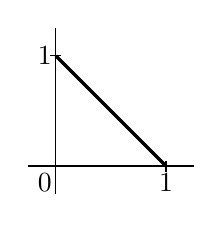
\begin{tikzpicture}[auto,scale = 0.7]
\draw (-0.5,0) -- (2.5,0);
\draw (0,-0.5) -- (0,2.5);
\draw (2,-0.1) -- (2,0.1);
\draw (-0.1,2) -- (0.1,2);
\node at (-0.2,-0.3) {0};
\node at (2,-0.3) {1};
\node at (-0.2,2) {1};
\draw [very thick] (2,0) -- (0,2);
\end{tikzpicture}
\begin{tikzpicture}
\draw[color = white] (0,-1) rectangle (0.7,-2);
\end{tikzpicture}
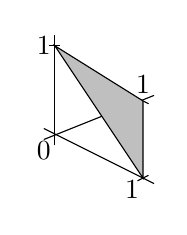
\begin{tikzpicture}[auto,scale = 0.7]
\draw (0,0) -- (0,2);
\draw (-0.2,0.1) -- (1.8,0.9);
\draw (-0.2,0.3) -- (1.8,-0.7);
\node at (-0.2,-0.1) {0};
\draw (-0.1,1.8) -- (0.1,1.8);
\node at (-0.2,1.8) {1};
\draw (1.5,-0.65) -- (1.7,-0.55);
\node at (1.4,-0.80) {1};
\draw (1.5,0.85) -- (1.7,0.75);
\node at (1.6,1.1) {1};
\draw[fill = gray!50] (0,1.8) -- (1.6,-0.6) -- (1.6,0.8) -- cycle;
\end{tikzpicture}
\begin{tikzpicture}
\draw[color = white] (0,-1) rectangle (0.7,-2);
\end{tikzpicture}
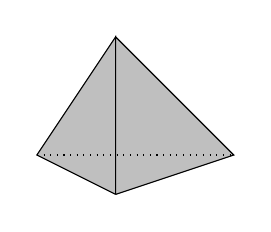
\begin{tikzpicture}[auto,scale = 1]
\node (0) at (0,0) {};
\node (1) at (-1,0.5) {};
\node (2) at (1.5,0.5) {};
\node (3) at (0,2) {};
\draw[fill = gray!50] (0,0) -- (-1,0.5) -- (0,2) -- (0,0);
\draw[fill = gray!50] (0,0) -- (1.5,0.5) -- (0,2) -- (0,0);
\draw[dotted] (-1,0.5) -- (1.5,0.5);
\end{tikzpicture}
				\caption{Standard geometric simplex $\Delta_0$, $\Delta_1$, $\Delta_2$, $\Delta_3$}
			\end{center}
			\end{figure}
		
		For $n \in \nat$ and $i \in \{0,\ldots, n+1\}$, let $\map{\partial_i}{\Delta_n}{\Delta_{n+1}}$ which maps $(t_0,\ldots,t_n)$ to $(t_0, \ldots, t_{i-1}, 0, t_i, \ldots, t_n)$. For $n \in \nat$ and $i \in \{0,\ldots, n\}$, let $\map{\xi_i}{\Delta_{n+1}}{\Delta_n}$ which maps $(t_0, \ldots, t_{n+2})$ to $(t_0, \ldots, t_{i-1}, t_i+t_{i+1}, t_{i+2}, \ldots, t_{n+2})$. This defines a functor $\map{G}{\Delta}{\topo}$ and so a functor $\map{Geom}{\sset}{\topo}$ called the \textbf{geometric realization}. It is always a CW-complex.
		
		The right adjoint of $Geom$, is called the \textbf{singular complex functor}, noted $\sing$, and is defined as follow. Given a topological space $X$, define $\sing(X)_n$ as the set of continuous functions from $\Delta_n$ to $X$. The face and degeneracy maps are:
		\begin{itemize}
			\item for $\map{\alpha}{\Delta_{n+1}}{X}$, $d_i(\alpha) = \alpha\circ\partial_i$,
			\item for $\map{\alpha}{\Delta_n}{X}$, $s_i(\alpha) = \alpha\circ\xi_i$.
		\end{itemize}
		
		\subsubsection{Kan complexes}
		\label{subsec:kancom}
		
		$\sing(X)$ always has a particular property: it is a \textbf{Kan complex}. Let us make precise this statement. Define the \textbf{standard simplex} $St^n$ to be the simplicial set $(St^n_m)_{m\in \mathbb{N}}$ with $St^n_m = \Delta(m,n)$, that is, the monotonous functions from $\{0, \ldots, m\}$ to $\{0, \ldots, n\}$. Its geometric realization is the standard geometric simplex. For $0 \leq i \leq n$, define the \textbf{$(n,i)$-horn} $\Lambda^{n,i}$ to be the sub-simplicial set of $St^n$ such that $\Lambda^{n,i}_m$ is the set of monotonous function $\map{f}{\{0,\ldots,m\}}{\{0,\ldots,n\}}$ such that $i$ is not in the image of $f$. Let $\map{\iota_i}{\Lambda^{n,i}}{St^n}$ denote the inclusion. 
		
		For example, in the case $n =2$, the geometric realizations of the standard simplex and of the horns are the following:
			\begin{figure}[H]
			\begin{center}
				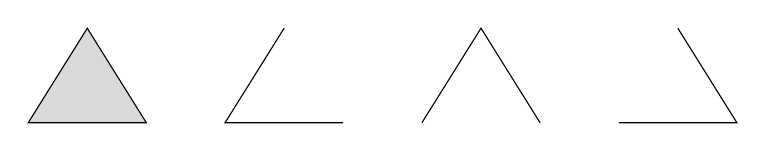
\begin{tikzpicture}[auto,scale = 1]

		\draw [fill=gray, fill opacity = 0.3] (0,0) -- (1.5,0) -- (0.75,1.2) -- cycle;
		\draw (3.25,1.2) -- (2.5,0) -- (4,0);
		\draw (5,0) -- (5.75,1.2) -- (6.5,0);
		\draw (7.5,0) -- (9,0) -- (8.25,1.2);
		
\end{tikzpicture}
				\caption{Geometric realizations of $St^2$, $\Lambda^{2,0}$, $\Lambda^{2,1}$, $\Lambda^{2,2}$}
			\end{center}
			\end{figure}
		
		A \textbf{Kan complex} is a simplicial set $X$ such that for every morphism $\map{f}{\Lambda^{n,i}}{X}$, there is a morphism $\map{\tilde{f}}{St_n}{X}$ which extends $f$, meaning that $\tilde{f}\circ\iota_i = f$. 
		
		The singular complex of a topological space is always a Kan complex. This comes from the fact that there is a retraction $\map{r}{Geom(St_n) = \Delta_n}{Geom(\Lambda^{n,i})}$. Indeed, $Geom(\Lambda^{n,i})$ is the subspace of $\Delta_n$ of points $(t_0, \ldots, t_n)$ such that there is a $j \neq i$ with $t_j = 0$. The retraction maps $(t_0,\ldots, t_n)$ to $(t_0 - s, \ldots, t_{i-1}-s, t_i+ns, t_{i+1}-s, \ldots, t_n-s)$ where $s = \min \{t_j \mid j \neq i\}$. 
		
		Kan complexes can model the expected behavior of $\infty$-groupoids: objects of dimension $0$ are element of $X_0$, morphisms are element of $X_1$, ... The existence of the inverse of a morphism $f \in X_1$ can be encoded by the Horn-filling condition. Start with the following horn:
			\begin{center}
				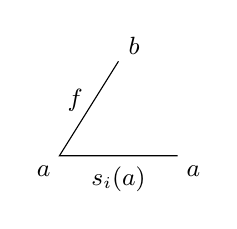
\begin{tikzpicture}[auto,scale = 1]

		\draw (3.25,1.2) -- (2.5,0) -- (4,0);
		\node (a) at (2.3,-0.2) {\small{$a$}};
		\node (f) at (2.7,0.7) {\small{$f$}};
		\node (b) at (3.45,1.4) {\small{$b$}};
		\node (s1a) at (3.25,-0.3) {\small{$s_i(a)$}};
		\node (aa) at (4.2,-0.2) {\small{$a$}};
		
\end{tikzpicture}
			\end{center}
		It can be extended to a $2$-simplex:
			\begin{center}
				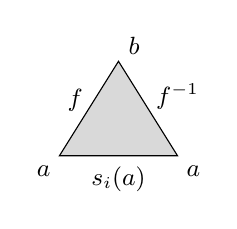
\begin{tikzpicture}[auto,scale = 1]

		\draw[fill=gray, fill opacity = 0.3] (3.25,1.2) -- (2.5,0) -- (4,0) -- cycle;
		\node (a) at (2.3,-0.2) {\small{$a$}};
		\node (f) at (2.7,0.7) {\small{$f$}};
		\node (b) at (3.45,1.4) {\small{$b$}};
		\node (s1a) at (3.25,-0.3) {\small{$s_i(a)$}};
		\node (aa) at (4.2,-0.2) {\small{$a$}};
		\node (fm1) at (4,0.75) {\small{$f^{-1}$}};
		
\end{tikzpicture}
			\end{center}
		Similarly, in the other way, which gives one an inverse modulo objects of dimension $2$, and this can be generalized to any dimension.
		
		
		\subsubsection{Kan-Quillen model structure and homotopy hypothesis}
		
		With this as an interpretation of $\infty$-groupoids, the homotopy hypothesis becomes a theorem:
		
		\begin{theo}[\cite{quillen67}]
		There is a model structure on $\sset$, called the \textbf{Kan-Quillen model structure} such that the adjunction $Geom \dashv \sing$ is a Quillen equivalence between the Quillen-Serre model structure on $\topo$ and this model category.
		\end{theo}
		
		The weak-equivalences of this model category are the morphisms $f$ of simplicial sets such that $Geom(f)$ is a weak homotopy equivalence. The fibrant and cofibrant objects are exactly the Kan complexes. This explains why the homotopy types of spaces are the same as Kan complexes, that is, $\infty$-groupoids.
		
		
		%d�finition des ensembles simpliciaux, des complexes de Kan, pourquoi �a mod�lise les infty-groupoides intuitivement
		
		%adjonction r�alisation-complexe singulier, �a d�finit des �quivalence faible sur les ensembles simpliciaux d'une ccat�gorie de mod�les, et qui rends l'adjonction une �quivalence de Quillen. C'est l'homotopy hypothesis.
	
	
	
\section{Model structures for $(\infty,1)$-categories and first attempt}

	
	We have seen in the previous section that topological spaces can be studied as $\infty$-groupoids. Almost the same should hold for d-spaces: d-spaces give rise to a natural structure of $\infty$-category. Objects of dimension $0$ are points, objects of dimension $1$ are dipaths, objects of dimension $2$ are dihomotopies, and so on. The only difference is that everything is not invertible: we have already seen that dipaths do not have an inverse modulo dihomotopy in general. But since we consider a dihomotopy as being a path in a topological space of paths, the $\infty$-groupoidal structure of those spaces transfers to the $\infty$-categorical structure of the d-space. More practically, dipaths are not invertible, but all the data of higher dimensions are invertible. To summarize, a d-space gives rise to a natural structure of an $(\infty,1)$-category, that is $1$-dimensional data is not reversible but higher dimensional data is.

	\subsection{Bergner model structure}
	
	
	As we have seen, the intuition is that an $(\infty,1)$-category is an $\infty$-category whose $1$-skeleton is a category with no particular property (at least, not a groupoid), and whose higher dimensional data between two objects of dimension $0$ has an $\infty$-groupoid structure. That is why, it is natural to model $(\infty,1)$-categories as ``categories enriched in $\infty$-groupoids''.
	
	Let us recall a few definitions from enriched categories. Let $\V$ be a monoidal category. We note $\otimes$ its tensor product, $I$ its unit element, $\map{\alpha_{a,b,c}}{(a\otimes b)\otimes c}{a\otimes(b\otimes c)}$ its associativity morphism, $\map{\lambda_a}{a\otimes a}{a}$ its left unit and $\map{\rho_a}{a\otimes a}{a}$ its right unit. In the following, we will use mainly categories ($\setcat$, $\sset$, $\Ab$, $\topo$, $\hotop$) with their cartesian structures.
	
	A (small) \textbf{enriched category $\C$ in $\V$} is the following data:
	\begin{itemize}
		\item a set $\ob{\C}$ (of \textbf{objects}),
		\item for every pair $(a,b)$ of objects, an object $\C(a,b)$ in $\V$,
		\item for every triple $(a,b,c)$ of objects, a morphism
		$$\map{\circ_{a,b,c}}{\C(a,b)\otimes\C(b,c)}{\C(a,c)}$$
		of $\V$, called the \textbf{composition},
		\item for every object $a$, a morphism
		$$\map{u_a}{I}{\C(a,a)}$$
		of $\V$, called the \textbf{unit}.
	\end{itemize}
	satisfying that:
	\begin{itemize}
		\item \textbf{(associativity axiom):} for every tuple $(a,b,c,d)$ of objects, the following diagram commutes:
		
		 \begin{center}
   			 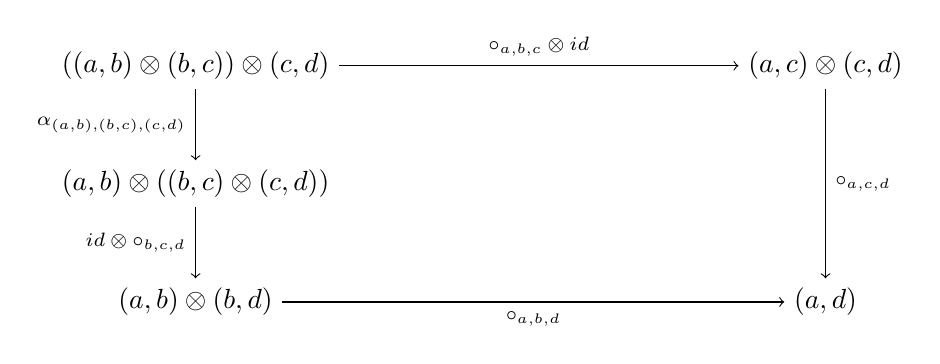
\begin{tikzpicture}[scale = 1]
  				\node (ABBC-CD) at (0,3) {$(\C(a,b)\otimes \C(b,c))\otimes \C(c,d)$};
      				\node (AB-BCCD) at (0,1.5) {$\C(a,b)\otimes (\C(b,c)\otimes \C(c,d))$};
      				\node (ABBD) at (0,0) {$\C(a,b)\otimes \C(b,d)$};
      				\node (ACCD) at (8,3) {$\C(a,c)\otimes \C(c,d)$};
      				\node (AD) at (8,0) {$\C(a,d)$};
     				\path[->,font=\scriptsize]
					(ABBC-CD) edge node[left]{$\alpha_{\C(a,b),\C(b,c),\C(c,d)}$} (AB-BCCD)
					(AB-BCCD) edge node[left]{$\text{id}\otimes \circ_{b,c,d}$} (ABBD)
					(ABBC-CD) edge node[above]{$\circ_{a,b,c}\otimes \text{id}$} (ACCD)
					(ACCD) edge node[right]{$\circ_{a,c,d}$} (AD)
					(ABBD) edge node[below]{$\circ_{a,b,d}$} (AD);
    			\end{tikzpicture}
 		 \end{center}
		
		\item \textbf{(unit axiom):} for every pair $(a,b)$ of objects, the following diagram commutes:
		
		\begin{center}
    			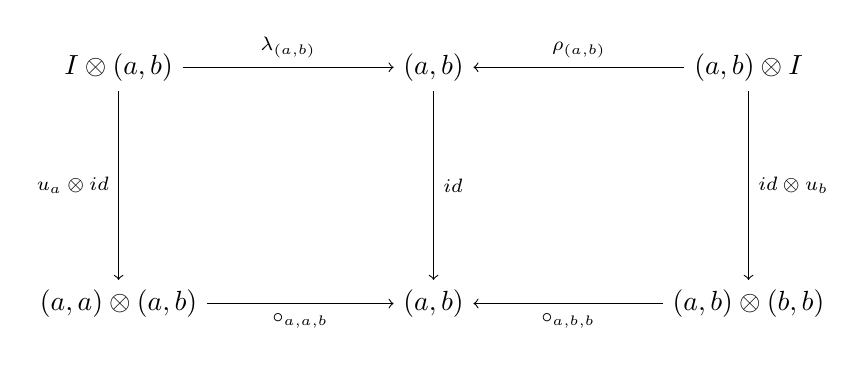
\begin{tikzpicture}[scale = 1]
      				\node (IAB) at (0,3) {$I\otimes\C(a,b)$};
       				\node (AAAB) at (0,0) {$\C(a,a)\otimes\C(a,b)$};
      				\node (ABt) at (4,3) {$\C(a,b)$};
      				\node (ABb) at (4,0) {$\C(a,b)$};
      				\node (ABI) at (8,3) {$\C(a,b)\otimes I$};
      				\node (ABBB) at (8,0) {$\C(a,b)\otimes\C(b,b)$};
      				\path[->,font=\scriptsize]
					(IAB) edge node[left]{$u_a \otimes \text{id}$} (AAAB)
					(IAB) edge node[above]{$\lambda_{\C(a,b)}$} (ABt)
					(AAAB) edge node[below]{$\circ_{a,a,b}$} (ABb)
					(ABt) edge node[right]{$\text{id}$} (ABb)
					(ABI) edge node[right]{$\text{id} \otimes u_b$} (ABBB)
					(ABI) edge node[above]{$\rho_{\C(a,b)}$} (ABt)
					(ABBB) edge node[below]{$\circ_{a,b,b}$} (ABb);
    			\end{tikzpicture}
  		\end{center}	
	\end{itemize}
\noindent An \textbf{enriched functor $F$ on $\V$} from $\C$ to $\D$ is the following data:
	\begin{itemize}
		\item a function $\map{F}{\ob{\C}}{\ob{\D}}$,
		\item for every pair $(a,b)$ of objects of $\C$, a morphism $\map{F_{a,b}}{\C(a,b)}{\D(F(a),F(b))}$ of $\V$,
	\end{itemize}
	satisfying that:
	\begin{itemize}
		\item for every triples $(a,b,c)$ of objects, the following diagram commutes:
		
		\begin{center}
    			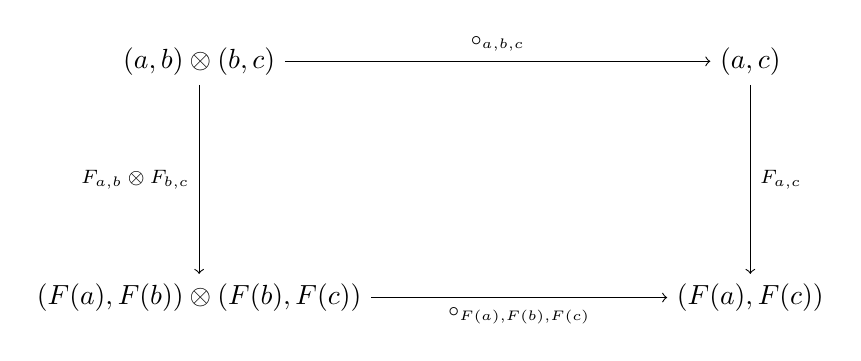
\begin{tikzpicture}
      				\node (ABBC) at (0,3) {$\C(a,b)\otimes\C(b,c)$};
       				\node (FAFBFBFC) at (0,0) {$\D(F(a),F(b))\otimes\D(F(b),F(c))$};
      				\node (AC) at (7,3) {$\C(a,c)$};
      				\node (FAFC) at (7,0) {$\D(F(a),F(c))$};
      				\path[->,font=\scriptsize]
					(ABBC) edge node[left]{$F_{a,b}\otimes F_{b,c}$} (FAFBFBFC)
					(ABBC) edge node[above]{$\circ_{a,b,c}$} (AC)
					(FAFBFBFC) edge node[below]{$\circ_{F(a),F(b),F(c)}$} (FAFC)
					(AC) edge node[right]{$F_{a,c}$} (FAFC);
    			\end{tikzpicture}
  		\end{center}
		
		\item for every object $a$ of $\C$, the following diagram commutes:
		
		\begin{center}
    			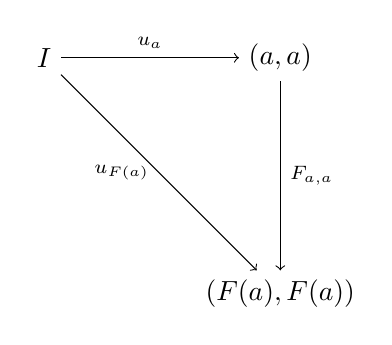
\begin{tikzpicture}
      				\node (I) at (0,3) {$I$};
       				\node (AA) at (3,3) {$\C(a,a)$};
      				\node (FAFA) at (3,0) {$\D(F(a),F(a))$};
     				\path[->,font=\scriptsize]
					(I) edge node[left]{$u_{F(a)}$} (FAFA)
					(I) edge node[above]{$u_a$} (AA)
					(AA) edge node[right]{$F_{a,a}$} (FAFA);
    			\end{tikzpicture}
  		\end{center}
		
	\end{itemize}
\noindent We note $\enrcat{\V}$ the category of enriched categories on $\V$ and enriched functors.
	
	For the rest of the subsection, let $\V = \sset$ with its cartesian structure. In this case, enriched categories are called \textbf{simplicial categories}. Given a simplicial category $\C$, one can define its $1$-skeleton $\tau_1(\C)$ as follow. First, given a simplicial set $X$, let $\pi_0(X)$ be the set $X_0/ \sim$ where $\sim$ is the smallest equivalence relation such that for every $c \in X_1$, $d_0(c) \sim d_1(c)$. $\pi_0$ extends to a functor from $\sset$ to $\setcat$, which preserves finite products. Define then $\tau_1(\C)$ the category whose:
	\begin{itemize}
		\item objects are objects of $\C$,
		\item morphisms from $a$ to $b$ are $\pi_0(\C(a,b))$,
		\item composition is given by $$\map{\pi_0(\circ_{a,b,c})}{\pi_0(\C(a,b))\times\pi_0(\C(b,c)) = \pi_0(\C(a,b)\times\C(b,c))}{\pi_0(\C(a,c))},$$
		\item the identity at $a$ is the equivalence class of the unique element of dimension $0$ in the image of $u_a$.
	\end{itemize}
	Intuitively, if we think $\C$ as a d-space, $\tau_1(\C)$ corresponds to its fundamental category. $\tau_1$ extends to a functor from $\enrcat{\sset}$ to $\cat$.
	
	There is then a model structure on $\enrcat{\sset}$, called the \textbf{Bergner model structure}, whose weak equivalences, called Dwyer-Kan weak equivalences in this context, are enriched functors $\map{F}{\C}{\D}$ such that:
	\begin{itemize}
		\item for every pair $(a,b)$ of objects of $\C$, $\map{F_{a,b}}{\C(a,b)}{\D(F(a),F(b))}$ is a weak equivalence in the Kan-Quillen model structure,
		\item $\tau_1(F)$ is an equivalence of categories.
	\end{itemize}
	See \cite{bergner04} for a complete description of this model category and proofs. As expected, the fibrant and cofibrant objects are simplicial categories whose hom-simplicial sets are Kan complexes, that is, $(\infty,1)$-categories.
	
	There are other model categories which are Quillen equivalent to Bergner's model structure. See, for example, the Joyal model structure on simplicial sets \cite{joyal08}, very close to the Kan-Quillen model structure.
	
	
	%intuition des infinie,1 cat et pourquoi c'est mieux pour mod�liser les d-spaces
	%cat�gorie enrichies au dessus de sset. pourquoi �a mod�lise les infty,1-cat. d�finition des �quivalences faibles. Evoquer la cat�gorie de mod�le de Joyal.
	
	
	\subsection{The trace and path categories}
	\label{subsec:trpacat}
	
	The idea for constructing a $(\infty,1)$-category from a d-space was to consider the category whose morphisms are dipaths. More precisely, the category whose:
	\begin{itemize}
		\item objects are points,
		\item morphisms from $a$ to $b$ are dipaths from $a$ to $b$, that is $\dipp{X}{a}{b}$,
		\item the identities are the constant dipath,
		\item composition is concatenation.
	\end{itemize}
	
The problem is that this is not a category since concatenation on dipaths is not associative. The idea from \cite{porter15} was to use traces instead. This category is called the \textbf{trace category} and denoted by $\trace{X}$. Since traces from $a$ to $b$ can be equipped with a topology which makes the concatenation continuous, this makes $\trace{X}$ a category enriched in $\topo$ with its cartesian structure. By applying the $Sing$ functor, this leads to a simplicial category, denoted by $\ttrace{X}$. The idea from \cite{porter08,porter15} was then to use tools from model categories to study d-spaces.

The first problem comes from the use of trace spaces instead of dipaths. We would expect that $\tau_1(\trace{X})$ to be (at least equivalent to) the fundamental category of $X$, which is not the case. The other problem is that comparing those simplicial categories up to Dwyer-Kan weak equivalences is an invariant of reversible equivalence by nature.

The first problem will be overcome by using dipaths instead of traces. Indeed, the concatenation is not associative, but it is modulo homotopy in the sense that the map $(\gamma_1,\gamma_2,\gamma_3) \mapsto \gamma_1\star(\gamma_2\star\gamma_3)$ is homotopic to the map $(\gamma_1,\gamma_2,\gamma_3) \mapsto (\gamma_1\star\gamma_2)\star\gamma_3$. To make this category of dipaths a category, we will consider it enriched in $\hotop$. We note $\dip{X}$ the category enriched in $\hotop$ defined above, with the exception that all continuous functions are taken modulo homotopy, that is:
	\begin{itemize}
		\item composition is concatenation modulo homotopy,
		\item the identity at $a$ is the homotopy class of the morphism from $\ast$, a one point space to $\dipp{X}{a}{a}$ which maps $\ast$ to the constant dipath.
	\end{itemize}
	
Dwyer-Kan weak equivalences can be modified in this context. First, the $1$-skeleton $\tau_1(\C)$ of an enriched category $\C$ in $\hotop$ is defined as follow:
	\begin{itemize}
		\item its objects are objects of $\C$,
		\item its morphisms from $a$ to $b$ are the path-connected components of $\C(a,b)$,
		\item composition is the function induced on path-connected components by the composition in $\C$.
	\end{itemize}
Since the path-connected components of $\dipp{X}{a}{b}$ are exactly the dihomotopy classes of dipaths, $\tau_1(\dip{X})$ is precisely the fundamental category $\funcat{X}$. We say \textbf{topological Dwyer-Kan weak equivalences} for the enriched functors $\map{F}{\C}{\D}$ between categories enriched in $\hotop$ such that:
	\begin{itemize}
		\item $F$ induces an equivalence of categories between the $1$-skeletons $\tau_1(\C)$ and $\tau_1(\D)$,
		\item for every pair $(a,b)$ of objects of $\C$, the map $\map{F_{a,b}}{\C(a,b)}{\D(F(a),F(b))}$ is an isomorphism of $\hotop$, that is, the homotopy class of a homotopy equivalence.
	\end{itemize}
	For a dimap $\map{f}{X}{Y}$, $\dip{f}$ is such a weak equivalence if and only if $f$ induces an equivalence of categories between fundamental categories and if for every pair $(a,b)$ of points of $\C$, the function $f_{a,b}$ from $\dipp{X}{a}{b}$ to $\dipp{Y}{f(a)}{f(b)}$ which maps $\gamma$ to $f\circ\gamma$ is a homotopy equivalence.
	
	\begin{theo}
	\label{theo:dkrev}
		If a dimap $\map{f}{X}{Y}$ is a reversible equivalence then $\dip{f}$ is a topological Dwyer-Kan equivalence.
	\end{theo}
	
	\begin{proof}
	The part for fundamental categories has already been proved in Corollary \ref{coro:revfun}.
	
	For the second part, fix $a$ and $b$ two points of $X$. We prove that $f_{a,b}$ is a homotopy equivalence. First note that if $\gamma$ is a reversible dipath from $a'$ to $a$ for some $a'$, the map $\gamma\star b$ from $\dipp{X}{a}{b}$ to $\dipp{X}{a'}{b}$ is a homotopy equivalence with inverse modulo homotopy $\gamma^{-1}\star b$. Idem for $\gamma$ from $b$ to $b'$ for some $b'$. Now let $\map{g}{Y}{X}$ and $\map{H}{X}{\rev{X}}$ a reversible homotopy with $H(x)(0) = x$ and $H(x)(1) = g\circ f(x)$. Then the following diagram is commutative modulo homotopy:
	
		\begin{center}
    			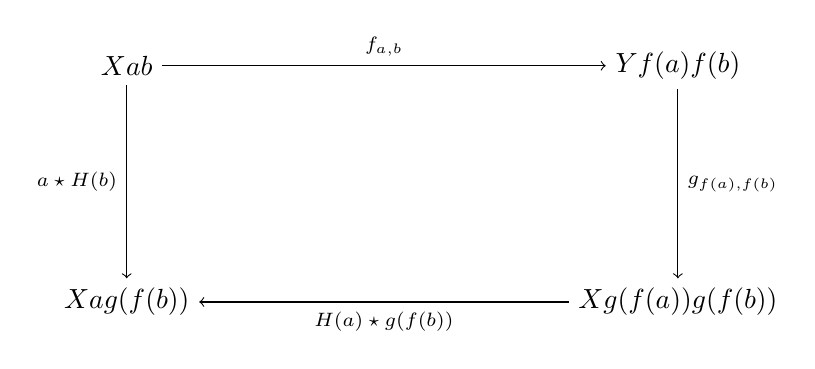
\begin{tikzpicture}
      				\node (ABBC) at (0,3) {$\dipp{X}{a}{b}$};
       				\node (FAFBFBFC) at (0,0) {$\dipp{X}{a}{g(f(b))}$};
      				\node (AC) at (7,3) {$\dipp{Y}{f(a)}{f(b)}$};
      				\node (FAFC) at (7,0) {$\dipp{X}{g(f(a))}{g(f(b))}$};
      				\path[->,font=\scriptsize]
					(ABBC) edge node[left]{$a\star H(b)$} (FAFBFBFC)
					(ABBC) edge node[above]{$f_{a,b}$} (AC)
					(FAFC) edge node[below]{$H(a)\star g(f(b))$} (FAFBFBFC)
					(AC) edge node[right]{$g_{f(a),f(b)}$} (FAFC);
    			\end{tikzpicture}
  		\end{center}
	the homotopy being the same as the one constructed in \ref{theo:brown}.
	
	Since $H(a)$ and $H(b)$ are reversible dipaths, and since homotopy equivalences have the 2-out-of-3 property, then $g_{f(a),f(b)}\circ f_{a,b}$ is a homotopy equivalence. Symmetrically, $f_{g(f(a)),g(f(b))}\circ g_{f(a),f(b)}$ is a homotopy equivalence. Consequently, $g_{f(a),f(b)}$ is a homotopy equivalence and so is $f_{a,b}$.
	\end{proof}
	
	
	Dipaths categories are then invariants of reversible equivalences modulo topological Dwyer-Kan equivalences, but not of other kind of ``dihomotopy equivalences''. We would be interested in the same kind of invariants for weaker equivalences. For example, as explained in the previous chapter, we would be interested in considering the category of components and not the fundamental category. Another problem to overcome is also the other condition of Dwyer-Kan equivalences. Indeed, requiring that for every pair of points $f_{a,b}$ is a homotopy equivalence between path spaces is also very strong. Consider a point space. Its dipath category has only one object and the dipath space is a point space. For a d-space, to have a Dwyer-Kan equivalence between its dipath category and the one of the point space requires in particular there is a dipath between every pair of points. In particular, essentially no pospace can fulfill this condition. The spaces which are equivalent to a point are the most simplest spaces one may consider, and one may expect that the basic bricks of the theory (for example, the $\Box_n$) to be equivalent to a point, which is not the case. In the next subsections, we will tackle this problem. One solution might have been to add the kind of equivalences we want using Bousfield localization on the Dwyer-Kan model category, but we will use another solution.
	
	\subsection{Partially enriched categories}
	\label{subsec:pec}
	
	We have seen that the problem comes from the mishandling of empty dipath spaces. We overcome this problem by explicitly handling them in the definition of an enriched category, leading to the notion of partially enriched categories. Those were invented (as far as I know) in \cite{dubut16b} in the case of Abelian groups to have an explicit ``empty group'' to define an analogue of the Grothendieck construction for diagrams with values in $\Ab$. We will see this later. A (small) \textbf{partially enriched category $\C$ in $\V$} is the following data:
	\begin{itemize}
		\item a set $\ob{\C}$ (of \textbf{objects}),
		\item a preorder $\leq$ on $\ob{\C}$, called the \textbf{domain},
		\item for every pair $a \leq b$ of objects, an object $\C(a,b)$ in $\V$,
		\item for every triple $a \leq b \leq c$ of objects, a morphism
		$$\map{\circ_{a,b,c}}{\C(a,b)\otimes\C(b,c)}{\C(a,c)}$$
		of $\V$, called the \textbf{composition},
		\item for every object $a$, a morphism
		$$\map{u_a}{I}{\C(a,a)}$$
		of $\V$, called the \textbf{unit}.
	\end{itemize}
	satisfying that:
	\begin{itemize}
		\item \textbf{(associativity axiom):} for every tuple $a \leq b \leq c \leq d$ of objects, the following diagram commutes:
		
		 \begin{center}
   			 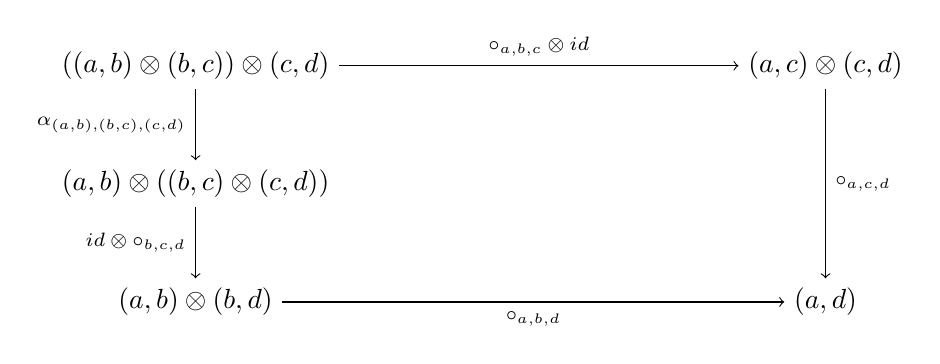
\begin{tikzpicture}[scale = 1]
  				\node (ABBC-CD) at (0,3) {$(\C(a,b)\otimes \C(b,c))\otimes \C(c,d)$};
      				\node (AB-BCCD) at (0,1.5) {$\C(a,b)\otimes (\C(b,c)\otimes \C(c,d))$};
      				\node (ABBD) at (0,0) {$\C(a,b)\otimes \C(b,d)$};
      				\node (ACCD) at (8,3) {$\C(a,c)\otimes \C(c,d)$};
      				\node (AD) at (8,0) {$\C(a,d)$};
     				\path[->,font=\scriptsize]
					(ABBC-CD) edge node[left]{$\alpha_{\C(a,b),\C(b,c),\C(c,d)}$} (AB-BCCD)
					(AB-BCCD) edge node[left]{$\text{id}\otimes \circ_{b,c,d}$} (ABBD)
					(ABBC-CD) edge node[above]{$\circ_{a,b,c}\otimes \text{id}$} (ACCD)
					(ACCD) edge node[right]{$\circ_{a,c,d}$} (AD)
					(ABBD) edge node[below]{$\circ_{a,b,d}$} (AD);
    			\end{tikzpicture}
 		 \end{center}
		
		\item \textbf{(unit axiom):} for every pair $a \leq b$ of objects, the following diagram commutes:
		
		\begin{center}
    			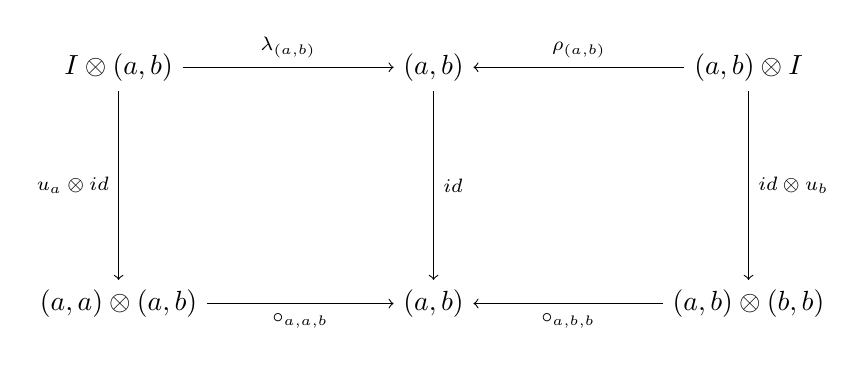
\begin{tikzpicture}[scale = 1]
      				\node (IAB) at (0,3) {$I\otimes\C(a,b)$};
       				\node (AAAB) at (0,0) {$\C(a,a)\otimes\C(a,b)$};
      				\node (ABt) at (4,3) {$\C(a,b)$};
      				\node (ABb) at (4,0) {$\C(a,b)$};
      				\node (ABI) at (8,3) {$\C(a,b)\otimes I$};
      				\node (ABBB) at (8,0) {$\C(a,b)\otimes\C(b,b)$};
      				\path[->,font=\scriptsize]
					(IAB) edge node[left]{$u_a \otimes \text{id}$} (AAAB)
					(IAB) edge node[above]{$\lambda_{\C(a,b)}$} (ABt)
					(AAAB) edge node[below]{$\circ_{a,a,b}$} (ABb)
					(ABt) edge node[right]{$\text{id}$} (ABb)
					(ABI) edge node[right]{$\text{id} \otimes u_b$} (ABBB)
					(ABI) edge node[above]{$\rho_{\C(a,b)}$} (ABt)
					(ABBB) edge node[below]{$\circ_{a,b,b}$} (ABb);
    			\end{tikzpicture}
  		\end{center}	
	\end{itemize}
 The axioms are the same as for enriched categories, except for the fundamental role played by the domain $\leq$ in every clause. Trivially, an enriched category is a partially enriched category whose domain is $\ob{\C}\times\ob{\C}$. One should note that partially enriched categories in $\topo$, in $\hotop$ and in $\sset$ are still very close to $(\infty,1)$-categories but also to Gaucher's flows \cite{gaucher03}, which were introduced for similar motivations. The dipath category is naturally a partially enriched categorie in $\hotop$ with the domain $\preceq$, called the \textbf{accessibility preordering}, defined as $a \preceq b$ if and only if there is a dipath from $a$ to $b$. A \textbf{partially enriched functor $F$ on $\V$} from $\C$ to $\D$ is the following data:
	\begin{itemize}
		\item a monotonous function $\map{F}{\ob{\C}}{\ob{\D}}$,
		\item for every pair $a \leq b$ of objects of $\C$, a morphism $\map{F_{a,b}}{\C(a,b)}{\D(F(a),F(b))}$ of $\V$,
	\end{itemize}
	satisfying that:
	\begin{itemize}
		\item for every triple $a \leq b \leq c$ of objects, the following diagram commutes:
		
		\begin{center}
    			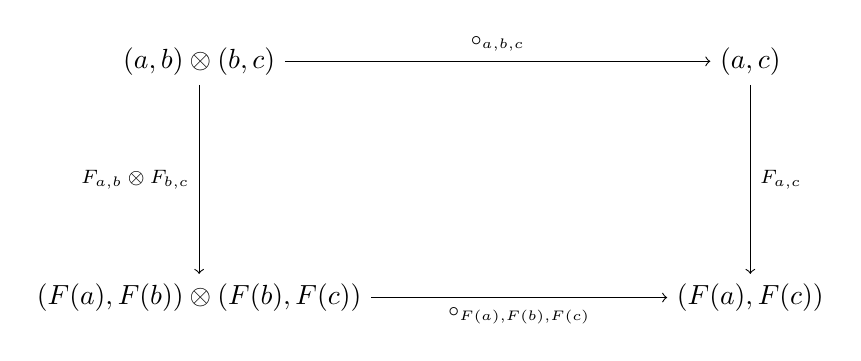
\begin{tikzpicture}
      				\node (ABBC) at (0,3) {$\C(a,b)\otimes\C(b,c)$};
       				\node (FAFBFBFC) at (0,0) {$\D(F(a),F(b))\otimes\D(F(b),F(c))$};
      				\node (AC) at (7,3) {$\C(a,c)$};
      				\node (FAFC) at (7,0) {$\D(F(a),F(c))$};
      				\path[->,font=\scriptsize]
					(ABBC) edge node[left]{$F_{a,b}\otimes F_{b,c}$} (FAFBFBFC)
					(ABBC) edge node[above]{$\circ_{a,b,c}$} (AC)
					(FAFBFBFC) edge node[below]{$\circ_{F(a),F(b),F(c)}$} (FAFC)
					(AC) edge node[right]{$F_{a,c}$} (FAFC);
    			\end{tikzpicture}
  		\end{center}
		
		\item for every object $a$ of $\C$, the following diagram commutes:
		
		\begin{center}
    			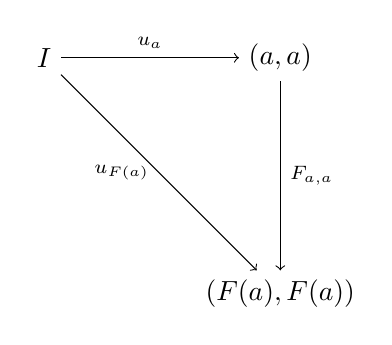
\begin{tikzpicture}
      				\node (I) at (0,3) {$I$};
       				\node (AA) at (3,3) {$\C(a,a)$};
      				\node (FAFA) at (3,0) {$\D(F(a),F(a))$};
     				\path[->,font=\scriptsize]
					(I) edge node[left]{$u_{F(a)}$} (FAFA)
					(I) edge node[above]{$u_a$} (AA)
					(AA) edge node[right]{$F_{a,a}$} (FAFA);
    			\end{tikzpicture}
  		\end{center}
		
	\end{itemize}
	
	We denote by $\pecat{\V}$ the category of partially enriched categories on $\V$ and partially enriched functors. $\overrightarrow{P}$ is then a functor from $\dtop$ to $\pecat{\hotop}$. The $1$-skeleton functor extends to $\pecat{\hotop}$: the only modification is that for every pair $a \not\leq b$ of objects of $\C$, the set of morphisms from $a$ to $b$ is the empty set. This leads to the category of components of a partially enriched category in $\hotop$, defined as $\comcat{\C} = \comcat{\tau_1{\C}}$. Note that the category of components of a d-space $X$, as defined in Section \ref{subsec:comcat}, is exactly $\comcat{\dip{X}}$. Note also that as previously, $\overrightarrow{\pi_0}$ is not a functor.
	
	We now can change the definition of weak-equivalences as desired. We say \textbf{inessential equivalence} for a partially enriched functor $\map{F}{\C}{\D}$ in $\hotop$ such that:
		\begin{itemize}
			\item $F$ induces an equivalence of categories between $\comcat{X}$ and $\comcat{Y}$,
			\item for every pair $a \leq b$ of objects of $\C$, $F_{a,b}$ is an isomorphism.
		\end{itemize}
		For a dimap $\map{f}{X}{Y}$, $\dip{f}$ is such an equivalence if and only if $f$ induces an equivalence of categories between component categories and if for every pair $a \leq b$ of points of $X$, the function $f_{a,b}$ from $\dipp{X}{a}{b}$ to $\dipp{Y}{f(a)}{f(b)}$ which maps $\gamma$ to $f\circ\gamma$ is a homotopy equivalence.
		
	
	%id�e: g�rer le vide explicitement -> cat�gories partiellemnt enrichies. d�f, d�f de foncteurs, exemple de la cat�gorie des chemins
	
	%\subsection{Weak equivalences}
	
	%on modifie la notion d'�quivalence faible on utilisant le cot� partiel. 
	
	
\section{Directed deformation retracts}

We can summarize what we have seen until now in the following array:
\begin{center}
\begin{tabular}{|c|c|c|c|}
  \hline
  type of equivalence & type of dipaths & localization of the fundamental category & weak equivalences\\
  \hline
  reversible & reversible & fundamental category/localizing isos & Dwyer-Kan \\
  \hline
  directed & all & groupoidification/localizing everything & none \\
  \hline
  ?? & ?? & component/localizing inessentials & inessential\\
  \hline
\end{tabular}
\end{center}

We would like now to complete this array by defining nice dipaths and equivalences that correspond to inessential equivalences. We will first define the type of dipaths we will use. The definition is very similar to the definition of inessential morphisms of a category. We will define the equivalence, but contrary to what we have seen with reversible and directed equivalences, we will not define them as inverse modulo the corresponding notion of dihomotopies, but using deformation retracts. Deformation retracts are a more intuitive way to define deformations of spaces and are enough to characterize homotopy equivalence.

	\subsection{Inessential dipaths}
	
	The class of dipaths we will consider are defined similarly to inessential morphisms of a category. First, we say that a dipath $\gamma$ from $a$ to $b$ is a \textbf{Yoneda dipath} if:
\begin{itemize}
	\item \textbf{right cancellation:} for every point $c$ such that $\dipp{X}{b}{c} \neq \varnothing$, the continuous function
	$$\gamma\star c : \dipp{X}{b}{c} \rightarrow \dipp{X}{a}{c} ~~~ \rho \mapsto \gamma\star\rho$$
	is a homotopy equivalence.
	\item \textbf{left cancellation:} for every point $c$ such that $\dipp{X}{c}{a} \neq \varnothing$, the continuous function
	$$c\star\gamma : \dipp{X}{c}{a} \rightarrow \dipp{X}{c}{b} ~~~ \rho \mapsto \rho\star\gamma$$
	is a homotopy equivalence.
\end{itemize}
We have seen that reversible dipaths are Yoneda and that was used to prove Theorem \ref{theo:dkrev}. On the other hand, the red dipath seen in the matchbox is not Yoneda.
The Ore conditions become the following. We say that a set $W$ of dipaths has:
\begin{itemize}
	\item \textbf{right Ore condition:} for every $\pale{\gamma}{a}{b} \in W$, for every dipath $\pale{\rho}{c}{b}$, there are $\pale{\gamma'}{d}{c} \in W$ and a dipath $\pale{\rho'}{d}{a}$ for some $d$ such that $\rho'\star\gamma$ is dihomotopic to $\gamma'\star\rho$
	\begin{center}
	\begin{tikzpicture}[scale=2]
		\node (A) at (0,1) {$d$};
		\node (B) at (1.2,1) {$a$};
		\node (C) at (0,0) {$c$};
		\node (D) at (1.2,0) {$b$};
		\node (E) at (0.6,0.5) {\scriptsize{mod. dihomot.}};
		\path[->,font=\scriptsize,dotted]
		(A) edge[snake it] node[above]{$\rho'$} (B)
		(A) edge[snake it] node[left]{$\gamma'\in W$} (C);
		\path[->,font=\scriptsize]
		(C) edge[snake it] node[below]{$\rho$} (D)
		(B) edge[snake it] node[right]{$\gamma\in W$} (D);
	\end{tikzpicture}
	\end{center}
	\item \textbf{left Ore condition:} for every $\pale{\gamma}{a}{b} \in W$ and every dipath $\pale{\rho}{a}{c}$ there are $\pale{\gamma'}{c}{d} \in W$ and a dipath $\pale{\rho'}{b}{d}$ for some $d$ such that $\gamma\star\rho'$ is dihomotopic to $\rho\star\gamma'$.
	\begin{center}
	\begin{tikzpicture}[scale=2]
		\node (A) at (0,1) {$a$};
		\node (B) at (1.2,1) {$c$};
		\node (C) at (0,0) {$b$};
		\node (D) at (1.2,0) {$d$};
		\path[->,font=\scriptsize]
		(A) edge[snake it] node[above]{$\rho$} (B)
		(A) edge[snake it] node[left]{$\gamma\in W$} (C);
		\path[->,font=\scriptsize,dotted]
		(C) edge[snake it] node[below]{$\rho'$} (D)
		(B) edge[snake it] node[right]{$\gamma'\in W$} (D);
	\end{tikzpicture}
	\end{center}
\end{itemize}

\begin{defi}
Given a d-space $X$, we define a \textbf{Yoneda system $\Theta$} of dipaths of $X$ as a subset of dipaths of $X$ such that:
\begin{itemize}
	\item every element of $\Theta$ is left and right cancellative,
	\item $\Theta$ has left and right Ore conditions.
\end{itemize}
\end{defi}

Similarly to Yoneda systems of morphisms, the set of Yoneda systems of dipaths is a complete lattice for inclusion (with $\sup$ as union). We denote by $\ine{X}$ the maximal Yoneda system of dipaths of $X$ and call its elements \textbf{inessential dipaths}.

\begin{lemme}
$\ine{X}$ contains the reversible dipaths, is closed under concatenation and dihomotopy.\\
Furthermore, $\{[\gamma] \mid \gamma \in \ine{X}\}$, the set of dihomotopy classes of elements of $\ine{X}$, is included in $\ine{\funcat{X}}$.
\end{lemme}

\begin{proof} ~
\begin{itemize}
	\item \textbf{$\ine{X}$ contains the reversible dipaths:} $\rev{X}$ is a Yoneda system.
	\item \textbf{$\ine{X}$ is closed under concatenation:} same proof as the closure under composition for $\ine{\C}$.
	\item \textbf{$\ine{X}$ is closed under dihomotopy:} since Yoneda dipaths are closed under dihomotopy and Ore conditions are modulo dihomotopy.
	\item $\{[\gamma] \mid \gamma \in \ine{X}\} \subseteq \ine{\funcat{X}}$: We prove that $\{[\gamma] \mid \gamma \in \ine{X}\}$ is a Yoneda system of morphisms of $\ine{\funcat{X}}$.
		\begin{itemize}
			\item \textbf{cancellation:} the map induced on path-connected components by $c\star\gamma$ is exactly $[\gamma]\circ c$. We have seen that a homotopy equivalence induces a bijection between path-connected components.
			\item \textbf{Ore condition:} easy.
		\end{itemize}
\end{itemize}
\end{proof}



	\subsection{Deformation retracts: non-directed and reversible cases}
	
	A deformation retract of a topological space is intuitively a subspace for which one can continuously deform the big space on the smaller space. Precisely, a pair $(X,A)$ of spaces with $A \subseteq X$ is a \textbf{deformation retract} if there is a homotopy $\map{H}{X}{\pathsp{X}}$ such that:
		\begin{itemize}
			\item $H(x)(0) = x$ for all $x \in X$,
			\item $H(x)(1) \in A$ for all $x \in X$,
			\item $H(a)(t) = a$ for all $a \in A$.
		\end{itemize}
One recovers homotopy equivalence as follow:

\begin{theo}[\cite{hatcher02}]
Two spaces $X$ and $Y$ are homotopically equivalent if and only if there are a space $Z$ and two deformation retracts $(Z,\tilde{X})$ and $(Z,\tilde{Y})$ with $X$ (resp. $Y$) homeomorphic to $\tilde{X}$ (resp. $\tilde{Y}$).
\end{theo}

The if part is easy since the map $x \mapsto H(x)(1)$ in the definition of a deformation retract is a homotopy equivalence with inverse the inclusion of $A$ in $X$. The converse uses the so-called \textbf{mapping cylinder}. Given a continuous function $\map{f}{X}{Y}$, define the space $M_f$ as the quotient $X\times[0,1] \sqcup Y$ by the relation such that for all $x \in X$, $(x,0)$ is equivalent to $f(x)$. Let $\tilde{X} = X\times\{1\}$ and $\tilde{Y} = Y$. Without any condition on $f$, it is easy to prove that $(M_f,\tilde{Y})$ is always a deformation retract. When furthermore $f$ is a homotopy equivalence, then $(M_f,\tilde{X})$ is also a deformation retract. See \cite{aguado12} for a complete (technical) description of the homotopy.

Actually, the very same construction works for reversible equivalence, as long as we equip the mapping cylinder with the suitable d-space structure. Given a dimap $\map{f}{X}{Y}$, define its \textbf{reversible mapping cylinder}, noted $\widetilde{M_f}$ as the quotient $X\times\revseg\sqcup Y$ by the same relation. Equivalently, it is defined as the d-space whose underlying space is $M_f$ and whose dipaths are generated by the dipaths of $Y$ and the paths $(\gamma,\gamma')$ of $X\times[0,1]$ where $\gamma$ is a dipath of $X$ and $\gamma'$ is any path.

Then a \textbf{reversible deformation retract} is a pair $(X,A)$ of d-spaces, where $A$ is a subd-space of $X$ (meaning that it is a subspace and the dipaths of $A$ are the dipaths of $X$ included in $A$), if there is a homotopy $\map{H}{X}{\rev{X}}$ such that:
		\begin{itemize}
			\item $H(x)(0) = x$ for all $x \in X$,
			\item $H(x)(1) \in A$ for all $x \in X$,
			\item $H(a)(t) = a$ for all $a \in A$, $t \in [0,1]$,
			\item $x \mapsto H(x)(t)$ is a dimap for all $t \in [0,1]$.
		\end{itemize}
Then $(\widetilde{M_f},\tilde{Y})$ is always a reversible deformation retract and when $f$ is a reversible equivalence, $(\widetilde{M_f},\tilde{X})$ is also a reversible deformation retract. Consequently:

\begin{theo}
\label{theo:drrev}
Two d-spaces $X$ and $Y$ are reversibly equivalent if and only if there are a d-space $Z$ and two reversible deformation retracts $(Z,\tilde{X})$ and $(Z,\tilde{Y})$ where $X$ (resp. $Y$) is dihomeomorphic to $\tilde{X}$ (resp. $\tilde{Y}$).
\end{theo}

The same argument does not work for directed equivalence, since the homotopy constructed in \cite{aguado12} uses the fact that one can reverse the time, which can be done in reversible dipaths, not in general.

	
%	\subsection{Directed extension}
%	
%	on peut faire la m�me chose avec les dichemins mais �a ne marche pas aussi bien.
%	
%	on aimerait compl�ter le tableau, on a besoin de chemin in�ssentiels
	
	\subsection{Inessential dipaths and deformations retracts}
	
	For the inessential case, we have a choice. Either use the homotopy equivalence framework, or use the deformation retract one, which a priori do not coincide. We choose to use the latter. Since inessential dipaths are not reversible in general, this leads to two notions of deformation retracts, depending on the direction of the deformation.
	
	We say that a pair $(X,A)$ of d-spaces is a \textbf{future inessential deformation retract} (FIDR for short) if there is a continuous function $\map{H}{X}{\ine{X}}$ ($\ine{X}$ is equipped with the subspace topology of $\dip{X}$) such that:
\begin{itemize}
	\item[--] for every $x \in X$, $H(x)(0) = x$,
	\item[--] for every $a \in A$ and $t \in [0,1]$, $H(a)(t) = a$,
	\item[--] for every $x \in X$, $H(x)(1) \in A$,
	\item[--] for every $t \in [0,1]$, the map $\map{H_t}{X}{X}$, $x \longmapsto H(x)(t)$ is a dimap,
	\item[--] for every dipath $\delta$ of $A$ from $z$ to $H_1(x)$ there is a dipath $\gamma$ of $X$ from $y$ to $x$ with $H_1(y) = z$ and $H_1\circ\gamma$ and $\delta$ are dihomotopic.
\end{itemize}
We stress here the fact that $H$ must take values in the inessential dipaths $\ine{X}$. Similarly, we define \textbf{past inessential deformation retracts} (PIDR for short) by switching the role of $1$ and $0$ in the previous definition. We then say that two d-spaces are \textbf{inessentially equivalent} if there is a zigzag of FIDR and PIDR between them.

\begin{exe}~
\label{exa:defret}
\begin{itemize}
	\item[1)] Observe that PIDR (resp. FIDR) between topological spaces (i.e. d-psaces whose set of dipaths contains all paths) coincide with non-directed deformation retracts. In particular, if two topological spaces are homotopically equivalent then they are inessentially equivalent. The converse also holds.
	\item[2)] $\{1\}$ is a future deformation retract of $\dirseg$. Indeed, the function $\map{H}{\dirseg}{\ine{\dirseg}}$, $s \longmapsto (t\longmapsto (1-t)s + t)$ satisfies the conditions above. Similarly, $\{0\}$ is a past deformation retract of $\dirseg$. More generally, every past face $\dirseg^k\times\{0\}\times\dirseg^l$ (resp. future face $\dirseg^k\times\{1\}\times\dirseg^l$) is a past (resp. future) deformation retract of the directed cube $\dirseg^{k+l+1}$.
	\item[3)] Is the deformation depicted in Section \ref{subsec:exa} a future deformation retract from $\matchbox$ to its upper face ? The answer is no because the dipaths followed by the homotopy are not all inessential. In particular, we have seen that the path on the back here:
			\begin{figure}[H]
			\begin{center}
				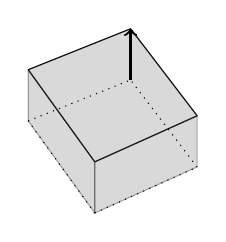
\begin{tikzpicture}[auto,scale = 0.65]
		\coordinate (A) at (0,0);
		\coordinate (B) at (2,0.9);
		\coordinate (C) at (-1.3,1.8);
		\coordinate (D) at (0.7,2.6);
		\coordinate (A') at (0,1);
		\coordinate (B') at (2,1.9);
		\coordinate (C') at (-1.3,2.8);
		\coordinate (D') at (0.7,3.6);
		\draw (A') -- (B');
		\draw (A') -- (C');
		\draw (B') -- (D');
		\draw (C') -- (D');
		\draw [fill = gray,draw = black,opacity = 0.3] (A) -- (B) -- (B') -- (A') -- (A);
		\draw [fill = gray,draw = black,opacity = 0.3] (A) -- (C) -- (C') -- (A') -- (A);
		\draw [fill = gray,draw = black,opacity = 0.3] (A') -- (B') -- (D') -- (C') -- (A');
		\draw[dotted](A) -- (B);
		\draw[dotted] (A) -- (C);
		\draw[dotted] (B) -- (D);
		\draw[dotted] (C) -- (D);
		\draw[->,thick] (D) -- (D');
		\end{tikzpicture}
			\end{center}
			\end{figure}
	is not inesential.
	\item[4)] We will see later that the category of components is an invariant of inessential equivalence, in the sense that if two d-spaces are inessentially equivalent, then they have equivalent categories of components. In particular, this implies that the matchbox $\matchbox$ is not inessentially equivalent to a point space, and that the Swiss flag SF is not inessentially equivalent to the squared annulus SA.
\end{itemize}
\end{exe}

\begin{prop}
If two d-spaces are reversibly equivalent, then they are inessentially equivalent. If two d-spaces are inessentially equivalent, then they are directedly equivalent.
\end{prop}

\begin{proof}
We use Theorem \ref{theo:drrev} for the first part. A reversible deformation retract is a FIDR (and modulo inversion of time, a PIDR). Indeed, the reversible dipaths are inessential and the last condition of a FIDR is automatic since $\gamma = \delta\star H(x)^{-1}$ works.

For the second part, if $(X,A)$ is a FIDR (or a PIDR), the inclusion of $A$ in $X$ is a directed equivalence with $H_1$ as inverse modulo directed homotopy.
\end{proof}

Finally, we can complete our array with the following:

\begin{theo}
A PIDR (resp. a FIDR) induces a inessential equivalence between dipath categories. Consequently, if two d-spaces are inessentially equivalent then their dipaths categories are inessentially equivalent.
\end{theo}

\begin{proof}
Let us prove the case of a FIDR. Note $H$ the homotopy and $H_t$ the d-map which maps $x$ to $H(x)(t)$. Let $\map{\iota}{A}{X}$ denote the inclusion. We will prove the following statements:
\begin{enumerate}
	\item for every pair $(a,b)$ of points of $A$ such that $\dipp{A}{a}{b} \neq \varnothing$, the function $\map{\iota_{a,b}}{\dipp{A}{a}{b}}{\dipp{X}{a}{b}}$ which maps $\gamma$ to $\gamma$ is a homotopy equivalence. And for every pair $(a,b)$ of points of $X$ such that $\dipp{X}{a}{b} \neq \varnothing$, the function $\map{H_{1,a,b}}{\dipp{X}{a}{b}}{\dipp{A}{H_1(a)}{H_1(b)}}$ which maps $\gamma$ to $H_1\circ\gamma$ is a homotopy equivalence.
	\item $H_1$ induces a functor $\comcat{H_1}$ from $\comcat{X}$ to $\comcat{A}$, i.e., if $\gamma \in \ine{\funcat{X}}$, then $H_1\circ\gamma \in \ine{\funcat{A}}$.
	\item the $\iota$ induces a functor $\comcat{\iota}$ from $\comcat{A}$ to $\comcat{X}$, i.e., $\ine{\funcat{A}} \subseteq \ine{\funcat{X}}$.
	\item $\comcat{H_1}$ and $\comcat{\iota}$ form an equivalence of categories.
\end{enumerate}
This implies that $\dip{\iota}$ and $\dip{H_1}$ are inessential equivalences.

Before starting, let us note the following about dihomotopies in $A$ and $X$:
\begin{itemize}
	\item two dipaths included in $A$ are dihomotopic in $A$ iff they are dihomotopic in $X$: the only if is trivial because a dihomotopy in $A$ is also a dihomotopy in $X$. The converse holds because a dihomotopy $K$ in $X$ between two dipaths $\gamma$, $\gamma'$ in $X$ induces a dihomotopy $H_1\circ K$ in $A$ between $H_1\circ\gamma = \gamma$ and $H_1\circ\gamma' = \gamma'$.
	\item for any pair $(a,b)$ of points of $A$, $\funcat{A}(a,b)$ is equal to $\funcat{X}(a,b)$: by the previous point, $\funcat{A}(a,b)$ embeds in $\funcat{X}(a,b)$. This injection is also surjective because any dipath $\gamma$ in $X$ between $a$ and $b$ is dihomotopic to $H_1\circ\gamma$.
\end{itemize}

\begin{enumerate}
	\item The proof is exactly the same as in theorem \ref{theo:brown}, the only property of the reversible dipaths used was the cancellation, which is also satisfied by inessential dipaths.
	\item We prove that $W = \{[H_1\circ\gamma] \mid [\gamma] \in \ine{\funcat{X}}\}$ is a Yoneda system of morphisms of $\funcat{A}$.
		\begin{itemize}
			\item \textbf{right cancellation:} let $\gamma$ be a dipath from $a$ to $b$ such that $[\gamma] \in \ine{\funcat{X}}$ and let $c \in A$ such that $\funcat{A}(H_1(b),c) \neq \varnothing$. We must prove that $$\map{(H_1\circ \gamma)\star c}{\funcat{X}(H_1(b),c)}{\funcat{X}(H_1(a),c)} ~~~ [\delta] \longmapsto [(H_1\circ\gamma)\star\delta]$$ is a bijection. The following diagram is commutative:
	\begin{center}
	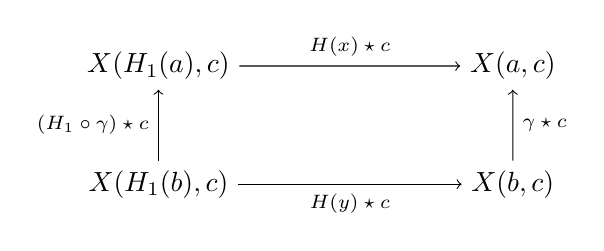
\begin{tikzpicture}[scale=1.5]
		\node (A) at (0,1) {$\funcat{X}(H_1(a),c)$};
		\node (B) at (3,1) {$\funcat{X}(a,c)$};
		\node (C) at (0,0) {$\funcat{X}(H_1(b),c)$};
		\node (D) at (3,0) {$\funcat{X}(b,c)$};
		\path[->,font=\scriptsize]
		(A) edge node[above]{$H(x)\star c$} (B)
		(D) edge node[right]{$\gamma\star c$} (B);
		\path[->,font=\scriptsize]
		(C) edge node[below]{$H(y)\star c$} (D)
		(C) edge node[left]{$(H_1\circ\gamma)\star c$} (A);
	\end{tikzpicture}
	\end{center}
	because $\gamma\star H(y)$ and $H(x)\star(H_1\circ\gamma)$ are dihomotopic. $H(x)\star c$ and $H(y)\star c$ are bijections because $H(x)$ and $H(y)$ belong to $\ine{X}$ and $\gamma\star c$ is a bijection because $[\gamma] \in \ine{\funcat{X}}$. $(H_1\circ\gamma)\star c$ is then a bijection.
			\item \textbf{left cancellation:} let $\gamma$ be a dipath from $a$ to $b$ such that $[\gamma] \in \ine{\funcat{X}}$ and let $c \in A$ such that $\funcat{A}(c,H_1(a)) \neq \varnothing$. We must prove that $$\map{c\star(H_1\circ \gamma)}{\funcat{X}(c,H_1(a))}{\funcat{X}(c,H_1(b))} ~~~ [\delta] \longmapsto [\delta\star(H_1\circ\gamma)]$$ is a bijection. Since $H(x) \in \ine{X}$, by the left Ore condition, there is dipath $\alpha$ from $d$ to $c$ for some $d$ such that $[\alpha] \in \ine{\funcat{X}}$ and $\funcat{X}(d,a) \neq \varnothing$. Consequently, the following diagram commutes:
			\begin{center}
	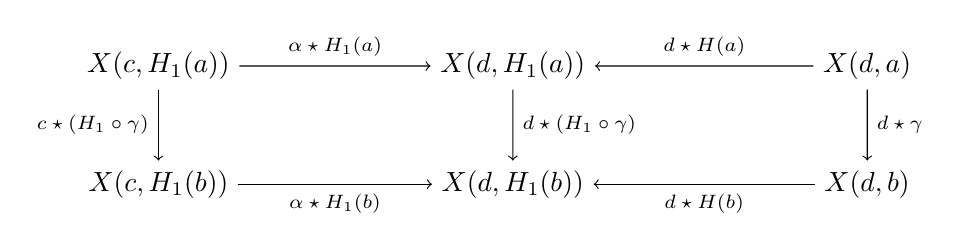
\begin{tikzpicture}[scale=1.5]
		\node (A) at (0,1) {$\funcat{X}(c,H_1(a))$};
		\node (B) at (3,1) {$\funcat{X}(d,H_1(a))$};
		\node (C) at (0,0) {$\funcat{X}(c,H_1(b))$};
		\node (D) at (3,0) {$\funcat{X}(d,H_1(b))$};
		\node (E) at (6,1) {$\funcat{X}(d,a)$};
		\node (F) at (6,0) {$\funcat{X}(d,b)$};
		\path[->,font=\scriptsize]
		(A) edge node[above]{$\alpha\star H_1(a)$} (B)
		(B) edge node[right]{$d\star(H_1\circ\gamma)$} (D)
		(E) edge node[right]{$d\star\gamma$} (F)
		(E) edge node[above]{$d\star H(a)$} (B)
		(F) edge node[below]{$d\star H(b)$} (D)
		(C) edge node[below]{$\alpha\star H_1(b)$} (D)
		(A) edge node[left]{$c\star(H_1\circ\gamma)$} (C);
	\end{tikzpicture}
	\end{center}
	$d\star\gamma$ is a bijection since $[\gamma] \in \ine{\funcat{X}}$ and $\funcat{X}(d,a) \neq \varnothing$. Similarly, $d\star H(a)$ and $d\star H(b)$ are bijections, so $d\star(H_1\circ\gamma)$ is a bijection. $\alpha\star H_1(a)$ and $\alpha\star H_1(b)$ are bijections because $\alpha \in \ine{\funcat{X}}$. Consequently, $c\star(H_1\circ\gamma)$ is a bijection.
			\item \textbf{right Ore condition:} let $[\gamma] \in \ine{\funcat{X}}$ with $\gamma$ a dipath from $a$ to $b$ and let $\delta$ be a dipath in $A$ from $c$ to $H_1(b)$. Since $H(b) \in \ine{X}$, $[\gamma\star H(b)] \in \ine{\funcat{X}}$. By the right Ore condition in $\funcat{X}$ on $[\gamma\star H(b)]$ and $[\delta]$ there are a dipath $\eta$ in $X$ from $d$ to $a$ and a dipath $\mu$ in $X$ from $d$ to $c$ such that $[\mu] \in \ine{\funcat{X}}$ and $\mu\star\delta$ is dihomotopic to $\eta\star\gamma\star H(b)$ and so to $\eta\star H(a)\star(H_1\circ\gamma)$. $\eta\star H(a)$ is dihomotopic to $H(d)\star (H_1\circ\eta)$ and since $c \in A$, $\mu$ is dihomotopic to $H(d)\star(H_1\circ\mu)$. $H(d)\star(H_1\circ\mu)\star\delta$ is dihomotopic to $H(d)\star(H_1\circ\eta)\star(H_1\circ\gamma)$. Since $H(d) \in \ine{X}$, $(H_1\circ\mu)\star\delta$ is dihomotopic to $(H_1\circ\eta)\star(H_1\circ\gamma)$ within $A$ and $[H_1\circ\mu] \in W$.
			\item \textbf{left Ore condition:} similar.
		\end{itemize}
	\item We start by proving that $W' = \{[\gamma] \mid [H_1\circ \gamma] \in \ine{\funcat{A}}\} \subseteq \ine{\funcat{X}}$. To this end, we prove that $W'' = \langle W' \cup \ine{\funcat{X}} \rangle$ is a Yoneda system (remember that $\langle W\rangle$ is the category generated by $W$).
		\begin{itemize}
			\item \textbf{right cancellation:} let $[\gamma] \in W'$, from $a$ to $b$ and let $c$ such that $\funcat{X}(b,c) \neq \varnothing$. Then, the following diagram commutes:
	\begin{center}
	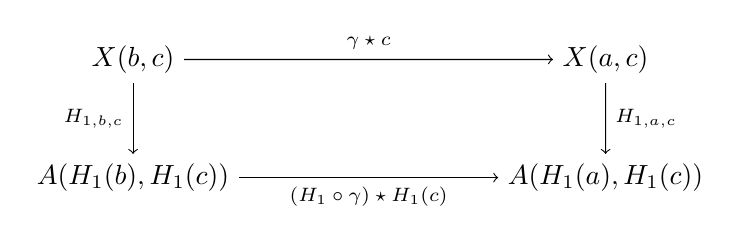
\begin{tikzpicture}[scale=1.5]
		\node (A) at (0,1) {$\funcat{X}(b,c)$};
		\node (B) at (4,1) {$\funcat{X}(a,c)$};
		\node (C) at (0,0) {$\funcat{A}(H_1(b),H_1(c))$};
		\node (D) at (4,0) {$\funcat{A}(H_1(a),H_1(c))$};
		\path[->,font=\scriptsize]
		(A) edge node[above]{$\gamma\star c$} (B)
		(B) edge node[right]{$H_{1,a,c}$} (D);
		\path[->,font=\scriptsize]
		(C) edge node[below]{$(H_1\circ\gamma)\star H_1(c)$} (D)
		(A) edge node[left]{$H_{1,b,c}$} (C);
	\end{tikzpicture}
	\end{center}
	We have already proved that $H_{1,b,c}$ and $H_{1,a,c}$ are homotopy equivalences and so induce bijections. $(H_1\circ\gamma)\star H_1(c)$ is a bijection since $H_1\circ\gamma \in \ine{\funcat{A}}$. Consequently, $\gamma\star c$ is a bijection.
			\item \textbf{left cancellation:} similar.
			\item \textbf{right Ore condition:} let $[\gamma] \in W'$ be a dipath from $a$ to $b$ and let $\delta$ be a dipath from $c$ to $b$. By the right Ore condition in $\funcat{A}$ between $H_1\circ\gamma$ and $H_1\circ\delta$, there are a dipath $\eta$ from $d$ to $H_1(a)$ and a dipath $\mu$ from $d$ to $H_1(c)$ such that $[\mu] \in \ine{\funcat{A}}$ and $\mu\star(H_1\circ\delta)$ is dihomotopic to $\eta\star(H_1\circ\gamma)$. Then, by the last condition of a FIDR, there is a dipath $\mu'$ from $e$ to $c$ such that $H_1\circ\mu'$ is dihomotopic to $\mu$ (and so $H_1(e) = d$). Since $H(a) \in \ine{X}$ then by the right Ore condition in $\funcat{X}$ between $H(a)$ and $H(e)\star\eta$, there are a dipath $\epsilon$ from $f$ to $e$ with $[\epsilon] \in \ine{\funcat{X}}$ and a dipath $\kappa$ from $f$ to $a$ such that $\epsilon\star H(e)\star \eta$ is dihomotopic to $\kappa\star H(a)$. Then $\kappa\star\gamma$ is dihomotopic to $\epsilon\star\mu'\star\delta$ with $[\epsilon\star\mu'] \in W''$.
			\item \textbf{left Ore condition:} let $[\gamma] \in W'$ be a dipath from $a$ to $b$ and let $\delta$ be a dipath from $a$ to $c$. By the left Ore condition in $\funcat{A}$ between $H_1\circ\gamma$ and $H_1\circ\delta$, there are a dipath $\eta$ from $H_1(b)$ to $d$ and a dipath $\mu$ from $H_1(c)$ to $d$ such that $[\mu] \in \ine{\funcat{A}}$ and $(H_1\circ\delta)\star\mu$ is dihomotopic to $(H_1\circ\gamma)\star\eta$. Then $\gamma\star(H(b)\star\eta)$ is dihomotopic to $\delta\star(H(c) \star\mu)$ with $[H(c)\star\mu] \in W''$.
		\end{itemize}
		
		We now prove that $\ine{\funcat{A}} \subseteq \ine{\funcat{X}}$. To this end, we prove that $W''' = \langle \ine{\funcat{A}}\cup\ine{\funcat{X}} \rangle$ is a Yoneda system.
			\begin{itemize}
				\item \textbf{right cancellation:} let $[\gamma] \in \ine{\funcat{A}}$, from $a$ to $b$ and let $c$ such that $\funcat{X}(b,c) \neq \varnothing$. Then, the following diagram commutes:
	\begin{center}
	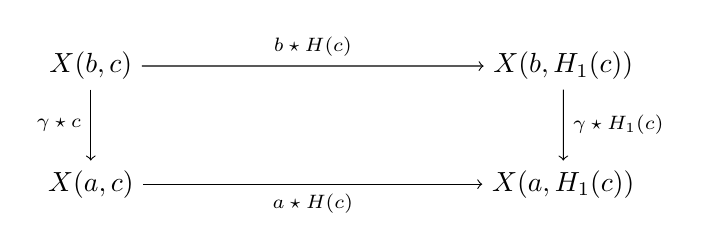
\begin{tikzpicture}[scale=1.5]
		\node (A) at (0,1) {$\funcat{X}(b,c)$};
		\node (B) at (4,1) {$\funcat{X}(b,H_1(c))$};
		\node (C) at (0,0) {$\funcat{X}(a,c)$};
		\node (D) at (4,0) {$\funcat{X}(a,H_1(c))$};
		\path[->,font=\scriptsize]
		(A) edge node[above]{$b\star H(c)$} (B)
		(B) edge node[right]{$\gamma\star H_1(c)$} (D);
		\path[->,font=\scriptsize]
		(C) edge node[below]{$a\star H(c)$} (D)
		(A) edge node[left]{$\gamma\star c$} (C);
	\end{tikzpicture}
	\end{center}
	$b\star H(c)$ and $a\star H(c)$ are bijection since $H(c) \in \ine{X}$ and $\gamma\star H_1(c)$ is a bijection since $\gamma \in \ine{\funcat{A}}$, $\funcat{X}(b,H_1(c)) = \funcat{A}(b,H_1(c))$ ($b \in A$) and $\funcat{X}(a,H_1(c)) = \funcat{A}(a,H_1(c))$ ($a \in A$). Consequently, $\gamma\star c$ is a bijection.
				\item \textbf{left cancellation:} similar.
				\item \textbf{right Ore condition:} let $[\gamma] \in \ine{\funcat{A}}$ with $\gamma$ a dipath in $A$ from $a$ to $b$. Let $\delta$ be a dipath in $X$ from $c$ to $b$. Then $\delta$ is dihomotopic to $H(c)\star (H_1\circ\delta)$, since $b \in A$. Since $H_1\circ\delta$ is a dipath in $A$ from $H_1(c)$ to $b$, then by the right Ore condition in $\funcat{A}$, there are a dipath $\eta$ from $d$ to $a$ and $\mu$ a dipath in $A$ from $d$ to $H_1(c)$ with $[\mu]\in\ine{\funcat{A}}$ and $\eta\star\gamma$ is dihomotopic to $\mu\star (H_1\circ\delta)$. By the last condition of a FIDR, there is a dipath $\mu'$ in $X$ from $e$ to $c$ with $H_1\circ\mu'$ is dihomotopic to $\mu$ (and so $H_1(e) = d$). $[\mu']$ belongs to $W' \subseteq \ine{\funcat{X}}$ and $\mu'\star\delta$ is dihomotopic to $\mu'\star H(c)\star(H_1\circ\delta)$ which is dihomotopic to $H(e)\star\mu\star(H_1\circ\delta)$ which is dihomotopic to $H(e)\star\eta\star\gamma$.
				\item \textbf{left Ore condition:} similar.
			\end{itemize}
	\item We have two functors $\map{\comcat{H_1}}{\comcat{X}}{\comcat{A}}$ and $\map{\comcat{\iota}}{\comcat{A}}{\comcat{X}}$. Let us prove that they form an equivalence of categories. First, $\comcat{H_1}\circ\comcat{\iota} = id_{\comcat{A}}$. Secondly, we have a natural transformation $\map{\nu}{id_{\comcat{X}}}{\comcat{\iota}\circ\comcat{H_1}}$ defined by $\map{\nu_x}{x}{H_1(x)} = [H(x)] \in \ine{\funcat{X}}$ and so is an isomorphism in $\comcat{X}$.
\end{enumerate}
\end{proof}


\section*{Conclusion}
	
To summarize, we have the following array:
\begin{center}
\begin{tabular}{|c|c|c|c|}
  \hline
  type of equivalence & type of dipaths & localization of the fundamental category & weak equivalences\\
  \hline
  reversible & reversible & fundamental category/localizing isos & Dwyer-Kan \\
  \hline
  directed & all & groupoidification/localizing everything & none \\
  \hline
  FIDR/PIDR & inessential & component/localizing inessentials & inessential\\
  \hline
\end{tabular}
\end{center}
In particular, we have described a new notion of dihomotopy equivalence using directed deformation retracts and inessential dipaths, that is, dipaths that have some properties of reversible ones. We prove that the action of inessential equivalence on fundamental categories corresponds to comparing categories of components up to equivalence. Furthermore, if reversible equivalence induces Dwyer-Kan weak equivalence on the dipath category, inessential equivalence induces something similar, up to two exceptions:
\begin{itemize}
	\item as said earlier, fundamental category is replaced by category of components,
	\item enriched categories are replaced by partially enriched categories allowing us to handle more carefully emptiness.
\end{itemize}











